\section{[WIP]Benutzerf"uhrung}

\subsection{[WIP]Elemente der grafischen Benutzeroberfl"ache}

\begin{figure}[htb]
\centering
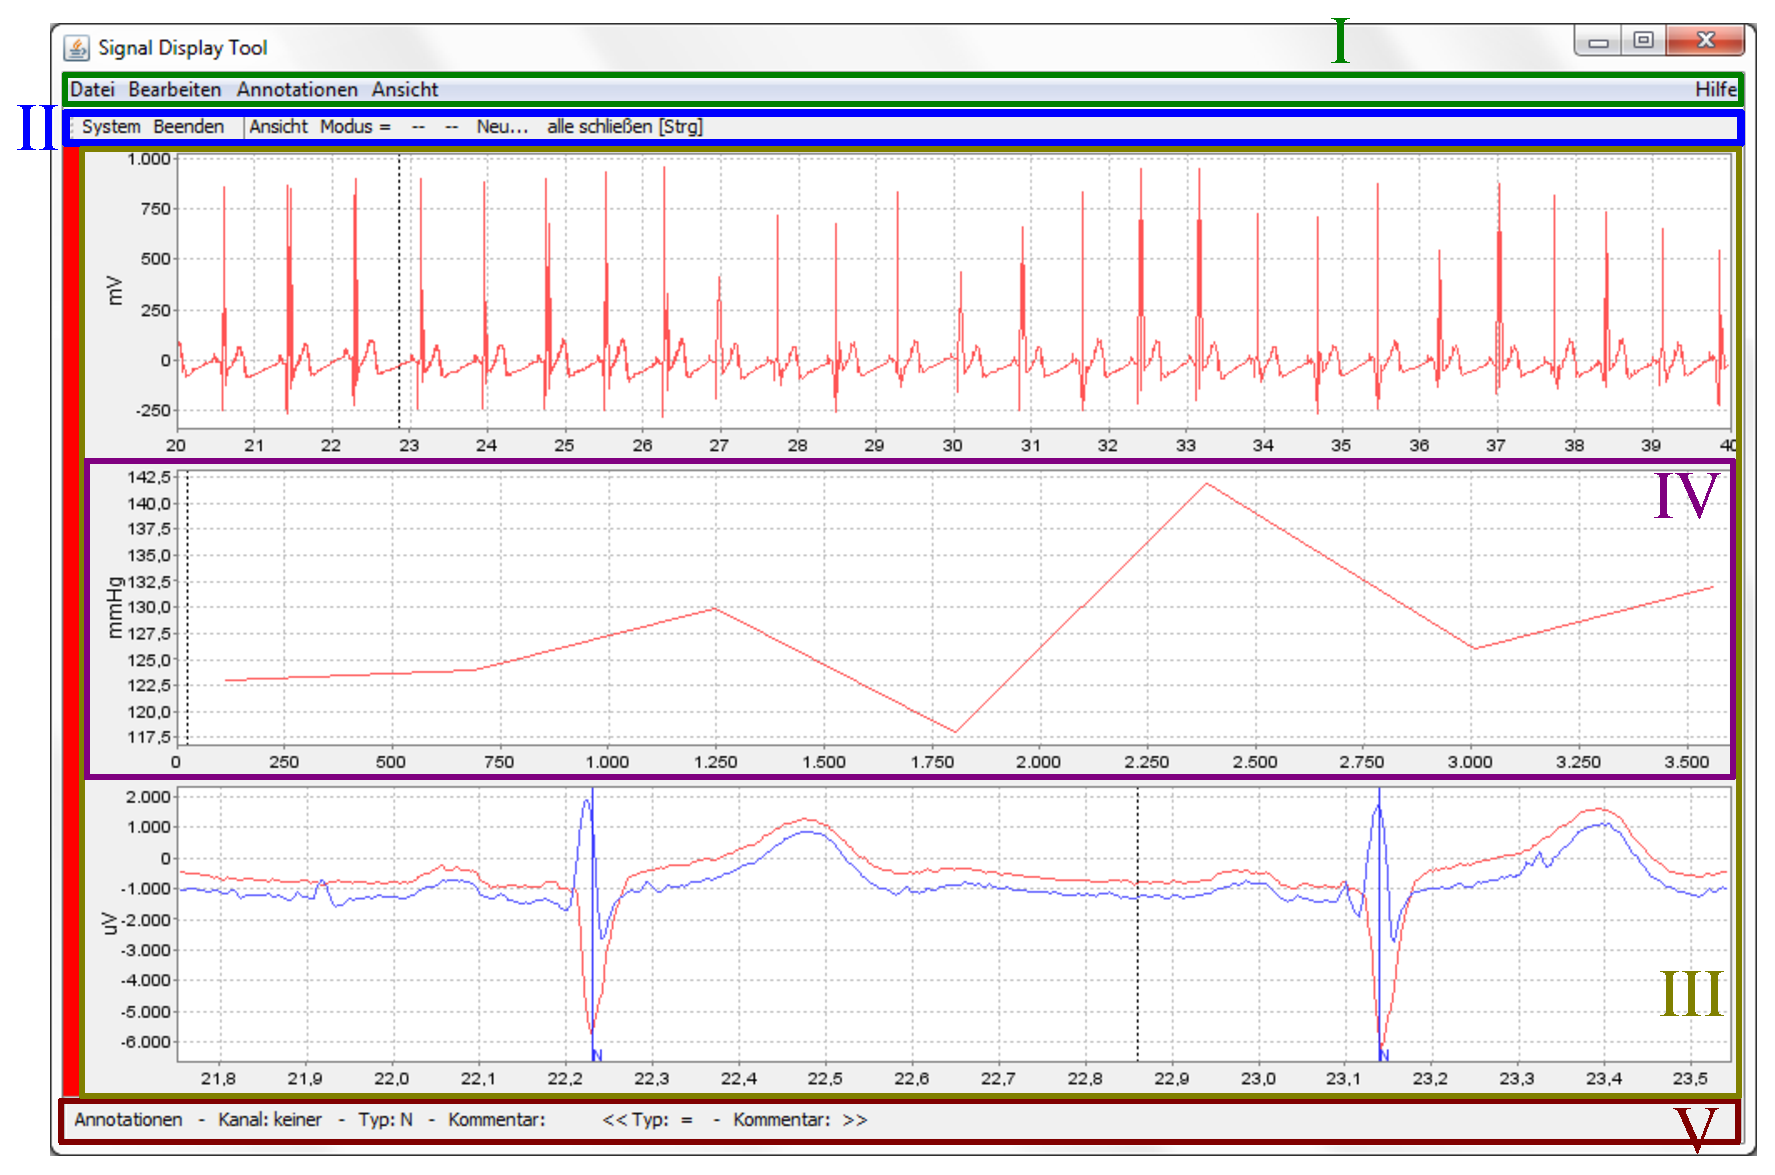
\includegraphics[width=\textwidth]{bilder/programm_ansicht.eps}
\caption[Klassen der grafischen Elemente]{Klassen der grafischen Elemente: I \texttt{Menus}, II \texttt{Toolbar}, III \texttt{SignalPanel}, IV \texttt{SignalView}, V \texttt{StatusBar}}
\label{pic:gui_elements_and_classes}
\end{figure}

\subsection{[WIP]Datenvisualisierung}

- Nutzung von JFreeChart (\ac{lgpl})

\subsection{[WIP]Umsetzung der \ac{GUI} im Paket \class{gst.ui}}

\begin{figure}[htb]
\centering
\includegraphics[angle=-90, width=0.9\textwidth]{bilder/package_ui_ubersicht.pdf}
\caption{"Ubersicht "uber das \class{ui}-Paket}
\label{pic:package_ui_ubersicht}
\end{figure}

- alle Elemente Singleton (bis auf \class{SignalView})

\subsubsection{[WIP]Koordiniertes Zoomen und Scrollen durch \class{SignalPanel}}

- Observer-Prinzip
- zwei eigene Managerklassen (Unabh"angigkeit)

\subsubsection{[WIP]Darstellung und Verarbeitung der Benutzereingaben}

- \class{SignalView} stellt dar
- Datenzugriff "uber abstrakte Definition von \class{DataController}
- Subklassen verarbeiten Maus- und Tastatureingabe

\subsubsection{[WIP]Verarbeitung und Ver"anderung von Annotationen}

- Einf"ugen von Annotationen "uber \class{AnnotationManager}
- Dreiecksbeziehung von \class{Annotation\-Controller}, \class{AnnotationList} und \class{AnnotationManager} erl"autern
- Suchalgorithmus zum finden der aktuellen Annotation
- "Anderung wird durch die Implementierung vom Interface \class{Data\-Change\-Listener} automatisiert aktualisiert
